\chapter{TC4合金固溶时效处理}
常见的\ti 钛合金热处理工艺有:退火、淬火(往往加上时效处理)、形变热处理等,不同的热处理方式得到的组织性能各异。现阶段\ti 合金的基本热处理工艺主要有:
\begin{enumerate}
	\item 固溶处理:实施固溶处理工艺,是为了得到等轴稳定的$\alpha $相、马氏体弥散的$ \alpha ^{\prime} $相、亚稳定状态的$\beta $相,等轴的$\alpha $相能够让合金的力学性能得到综合性的提升,马氏体弥散的$ \alpha ^{\prime} $相能够让合金,在强度、硬度上得到提高,塑性、韧性被降低\cite{gurong2002}。
	\item 时效处理:次生的$\alpha $相体积分数在TC4钛合金中,会对屈服强度产生很大的影响。在条件相等的情况之下,时效温度越低组织越小,时效温度高低组织越大。研究人员主要是通过控制参数,来影响对次生$\alpha $相的含量,从而实现TC4钛合金强度和塑性的匹配。
	\item 深冷处理:深冷处理是20世纪60年代以来兴起的一种新型冷处理工艺。通过对材料进行-130°C以下的低温处理,可以对金属内部的组织进行改善,并且能够让在热处理之后残留的奥氏体被清除掉。实验研究发现,原始的$\beta $相会在深冷处理的过程当中,逐渐的向$\alpha^{\prime} $相去转变,残余应力在组织中会变少,与此同时网篮状组织的增加,会让TC4钛合金的韧性、强度、塑性,在组织上的性能得到提高。
	\item 氮化处理:常在冷轧后进行氮化处理,TC4在低温氮化过程中会发生重结晶,可以避免晶粒粗化,提高表面强度\cite{guotanliuMicrostructureEvolutionTi2022}。
\end{enumerate}
不同的热处理工艺互相组合可以对合金产生更好的强化效果,现阶段工业上常采用\cite{zhoukaixiangJiyushenlengchulidenanjiagongcailiaoqiexiaotexingyanjiu2022}:淬火+时效;固溶+时效;双重固溶+时效;固溶+双重时效;时效+冷轧+低温氮化等,其中固溶+时效处理是应用最为广泛的一种热处理工艺组合。

对于$\alpha+\beta$型的\ti 钛合金的固溶时效热处理工艺而言,其主要影响参数为固溶、时效的温度和时间\cite{mirror1,ranxingGurongwenduduiTi6Al4VELItaihejinxianweizuzhijixingnengdeyingxiang2021}。


冉兴等人表明\cite{ranxingGurongwenduduiTi6Al4VELItaihejinxianweizuzhijixingnengdeyingxiang2021}在固溶温度为952℃附近时,TC4合金具有较高的强度,但随着温度的升高其脆性增加;鲁媛媛,马保飞等人研究发现在时效温度为450℃、500℃和550℃时初生α相的含量随温度升高逐渐增加;而在时效温度为600℃和650℃条件下初生$\alpha$相含量因高温溶解而明显减少, $\beta$相尺寸相应增大。当时效温度为550℃时, 所得钛合金的显微组织最佳\cite{luyuanyuanShixiaochuliduiTC4taihejinweiguanzuzhihelixuexingnengdeyingxiang2019}。刘婉颖、林元华等人通过实验发现:在960 ℃/1 h + WQ进行固溶处理和500 ℃/4 h + AC下进行时效处理得到的\ti 具有最佳的力学性能\cite{LiuWanYingBuTongReChuLiGongYiDuiTi6Al4VTaiHeJinWeiGuanJieGouHeLiXueXingNengYingXiangYingWen2017};陈冠宇通过实验表明,在850℃进行退火处理时,在600℃进行时效处理可以使合金得到更好的耐腐蚀性能\cite{1200};李宸宇证明\ti 合金在900℃空冷固溶两小时在530℃时效四小时后具有更好的强硬度,而且固溶后冷速越快,合金的强硬度越高、塑韧性越差\cite{900}。%第46页

根据对万能力学试验机上测试得到的数据进行整理,得到了抗拉强度\footnote{根据《金属材料室温拉伸试验方法》GBT228-2002,抗拉强度符号已经由$ R_m $代替旧国标中的$ \sigma_b $,故在此使用最新标准$ R_m $来表示抗拉强度。}、延伸率,如\ref{sec:mystrength}所示。又通过去除力学试验数据中从断裂瞬间到试验结束之间的无用数值、整合每组两个试验结果(取平均值),计算得到了如\ref{sec:mystrength}的实验结果:
\begin{table}[htbp]
	\centering
	\caption{\ti 合金的力学性能试验结果}
	\label{sec:mystrength}
	\begin{tabular}{ccccc}
		\toprule
		试验编号& 代号&$ R_m $(Mpa)&$ R_0.2 $(Mpa)&延伸率 \\
		\midrule
		0 & 甲 & 1008.69 &986.32& 6.83$\%$ \\
		1 & 乙 & 1188.36 &1054.61 &3.73$\%$ \\
		2 & 丙 & 1077.33 & 997.07&4.24$\%$ \\
		3 & 丁 & 1094.87 & 998.00&3.49$\%$ \\
		4 & 戊 & 1099.33 &986.20 &2.60$\%$ \\
		5 & 己 & 1113.90 & 1021.35&2.57$\%$ \\
		6 & 庚 & 1077.28 &992.31& 2.88$\%$ \\
		7 & 辛 & 790.10 & 脆断&1.94$\%$ \\
		8 & 壬 & 799.54 &脆断& 2.05$\%$ \\
		9 & 癸 & 873.38 & 脆断&2.19$\%$ \\
		\bottomrule
	\end{tabular}
\end{table}

通过室温力学拉伸试验,得到试样断裂区域截面($ 1.3mm\times2.5mm=3.25mm^2 $)的应力与应变曲线(拉伸变形量与拉伸区域长度的比值),将把包括未处理的对照组在内的十组数据的应力应变曲线进行汇总,得到了如\ref{fig:试样应力应变曲线汇总}\footnote{图形中标签未标明的,所有组共同具有工艺参数为:固溶处理时间10分钟;时效处理时间60分钟}所示的应力应变曲线汇总图:
\begin{figure}[h!]
	\centering
	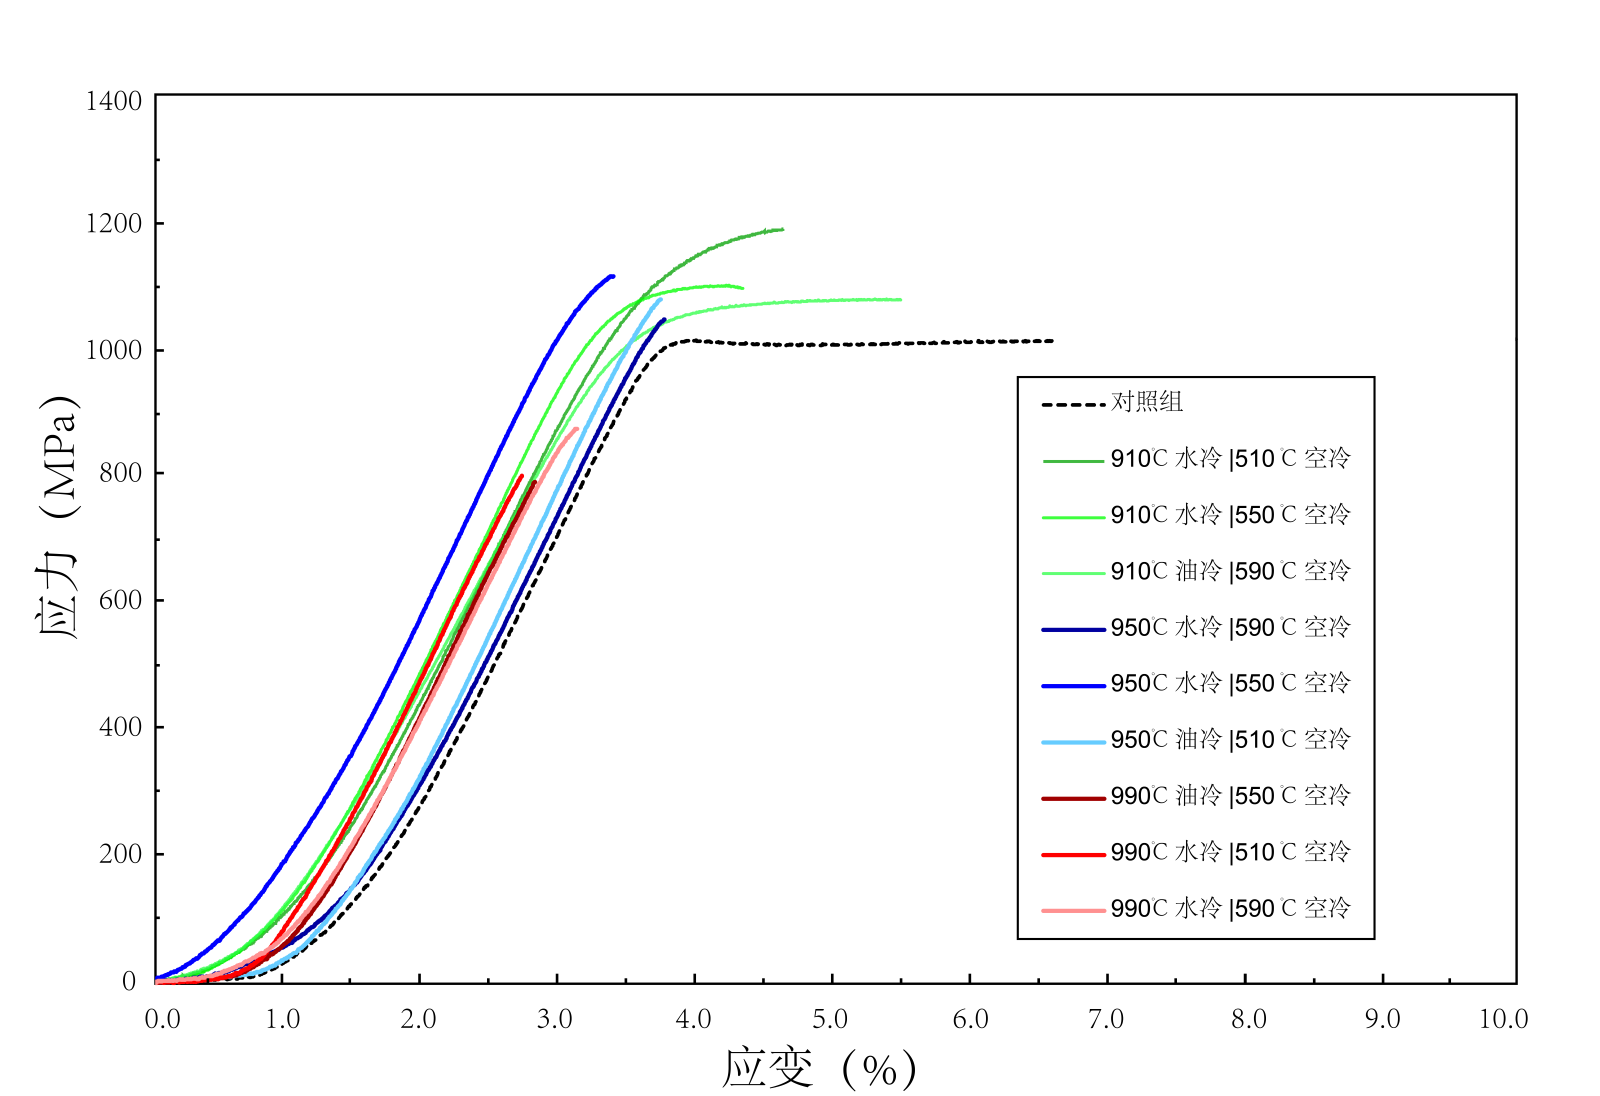
\includegraphics[width=0.99\linewidth]{pic/试样应力应变曲线汇总min.png}
	\caption{试样应力应变曲线汇总}
	\label{fig:试样应力应变曲线汇总}
\end{figure}
从图中经过分析可以看出:固溶-时效处理后试样对材料各方面的影响还是比较明显的。力学性能对比分析如下
\begin{enumerate}
	\item \textbf{整体塑性降低:}与对照组相比,910℃固溶组塑性大幅度降低,在经过短暂的屈服阶段后即被拉断;950℃、990℃固溶组的塑性更低,几乎呈现出来脆性材料的特点,断裂都属于脆性断裂。
	\item \textbf{抗拉强度有所提升:}910℃、950℃固溶组的抗拉强度与对照组相比都有所提升,其中以910℃固溶+510℃空冷组的强度为最高。
	\item \textbf{固溶温度较高时,强度有所降低}990℃固溶组的强度、塑性降低最为明显,990℃固溶+550℃空冷组的抗拉强度已经降低到了$ 790Mpa $左右,990℃固溶+510℃空冷组的最大应变达到了$ 2.18\% $,几乎是对照组$ 6.83\% $的三分之一。
\end{enumerate}


本设计设置的固溶处理的温度较高,在相变点附近,在高温状态下进行保温目的是为了让合金内部化学元素发生充分扩散,使成分均匀化,并发生 $\alpha\to\beta$ 转变以获得高温$ \beta $相组织。保温一段时间后,在较快冷却条件下抑制钛合金自发的$\beta\to \alpha$ 转变, 从而获得 $ \alpha^{\prime} $相马氏体、$ \alpha^{\prime\prime} $相马氏体以及亚稳$ \beta^{\prime} $相等组织。
%TC4 钛合金在稳定状态下含有少量的 β 相,β 相的存在使其具有热处理强化的能 力。由\ref{fig:tc4change}可知,固溶处理过程中固溶温度对固溶后的亚稳定相种类起决定作 用,不同固溶温度下 α 与 β 相的平衡体积分数不同,造成 β 相中合金元素含量不同, 从而在快速冷却过程中产生不同的亚稳定相。

\begin{figure}[h!]
	\centering
	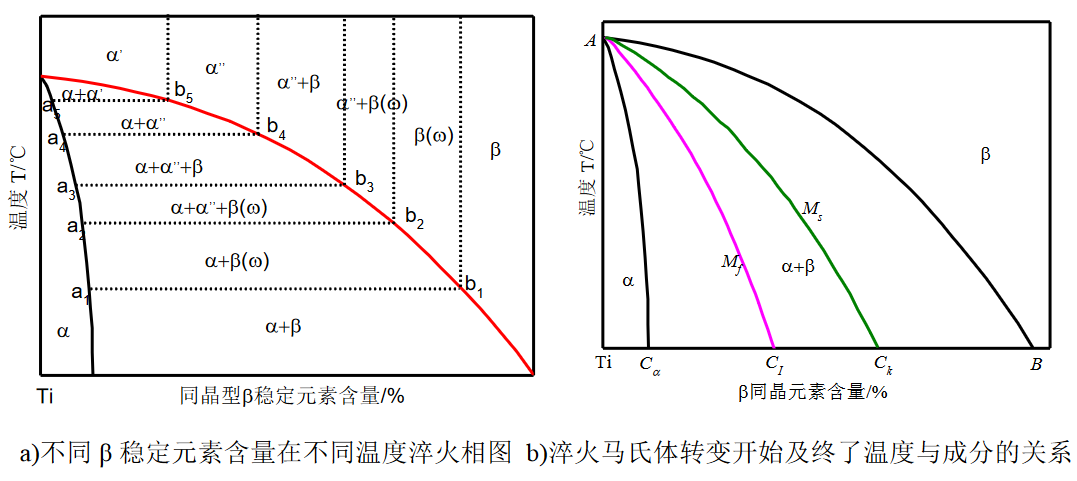
\includegraphics[width=0.7\linewidth]{pic/tc4change}
	\caption{钛合金在淬火过程中的亚稳定相及马氏体转变温度}
	\label{fig:tc4change}
\end{figure}

固溶处理得到的组织可以为后续的时效处理提供良好的组织状态。本实验时效处理的温度较低,在500℃附近,通过将固溶处理后得到的亚稳态组织加热到一定温度后保温60分钟,目的是促使得到的亚稳定相在热力学作用下来降低体系的能量,使组织向稳定状态转变,产生弥散分布的析出相,来对合金起到强化作用。

%在对拉伸试验的结果进行初步分析后,发现固溶与时效的处理对于合金性能的影响强度是不同的,其中以固溶处理对合金性能的影响较大,因此本实验以固溶温度为主要影响因素进行分析,将热处理的后的九组试样根据固溶温度(\textbf{510-550-590})分为三个大组来进行分析:

\section{相变点以下固溶处理对组织性能的影响}
			\begin{figure}[htbp]
				\centering
				\subfigure[910℃固溶(油冷)+590℃固溶]{
					\begin{minipage}[t]{0.33\linewidth}
						\centering
						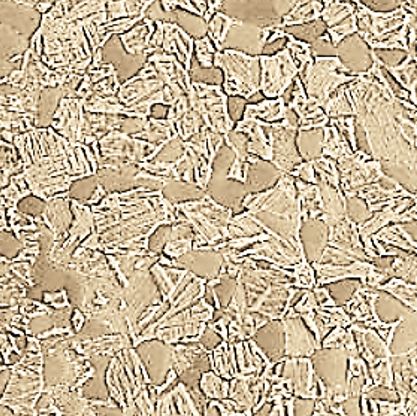
\includegraphics[width=0.9\linewidth]{pic/组织分析/910+590}
						\label{fig:910590}
					\end{minipage}%
				}%
				\subfigure[910℃固溶(水冷)+550℃固溶]{
				\begin{minipage}[t]{0.33\linewidth}
					\centering
					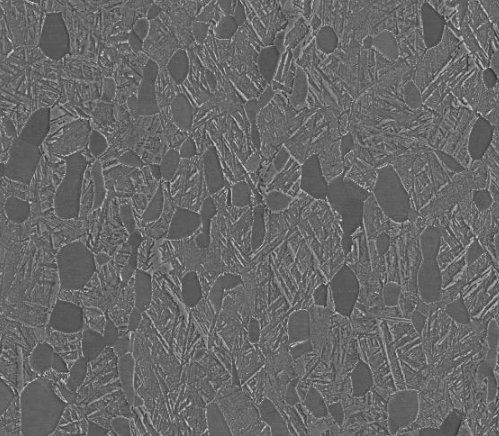
\includegraphics[width=0.9\linewidth]{pic/组织分析/910+550}
					\label{fig:910550}
					%\caption{fig2}
				\end{minipage}%
			}%
				\subfigure[910℃固溶(水冷)+510℃固溶]{
					\begin{minipage}[t]{0.33\linewidth}
						\centering
						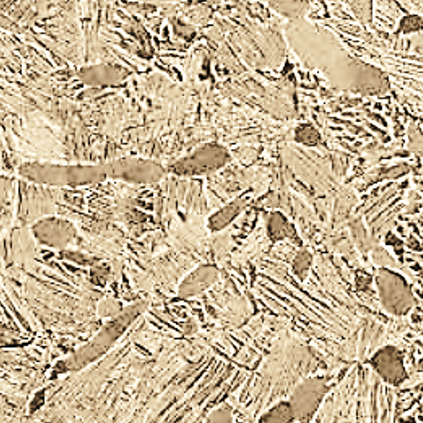
\includegraphics[width=0.9\linewidth]{pic/组织分析/910+510}
						\label{fig:910510}
						%\caption{fig2}
					\end{minipage}%
				}%
				\centering
				\label{910}
				\caption{不同冷却方式下的 TC4 钛合金显微组织}
			\end{figure}
			\begin{figure}[h!]
			\centering
			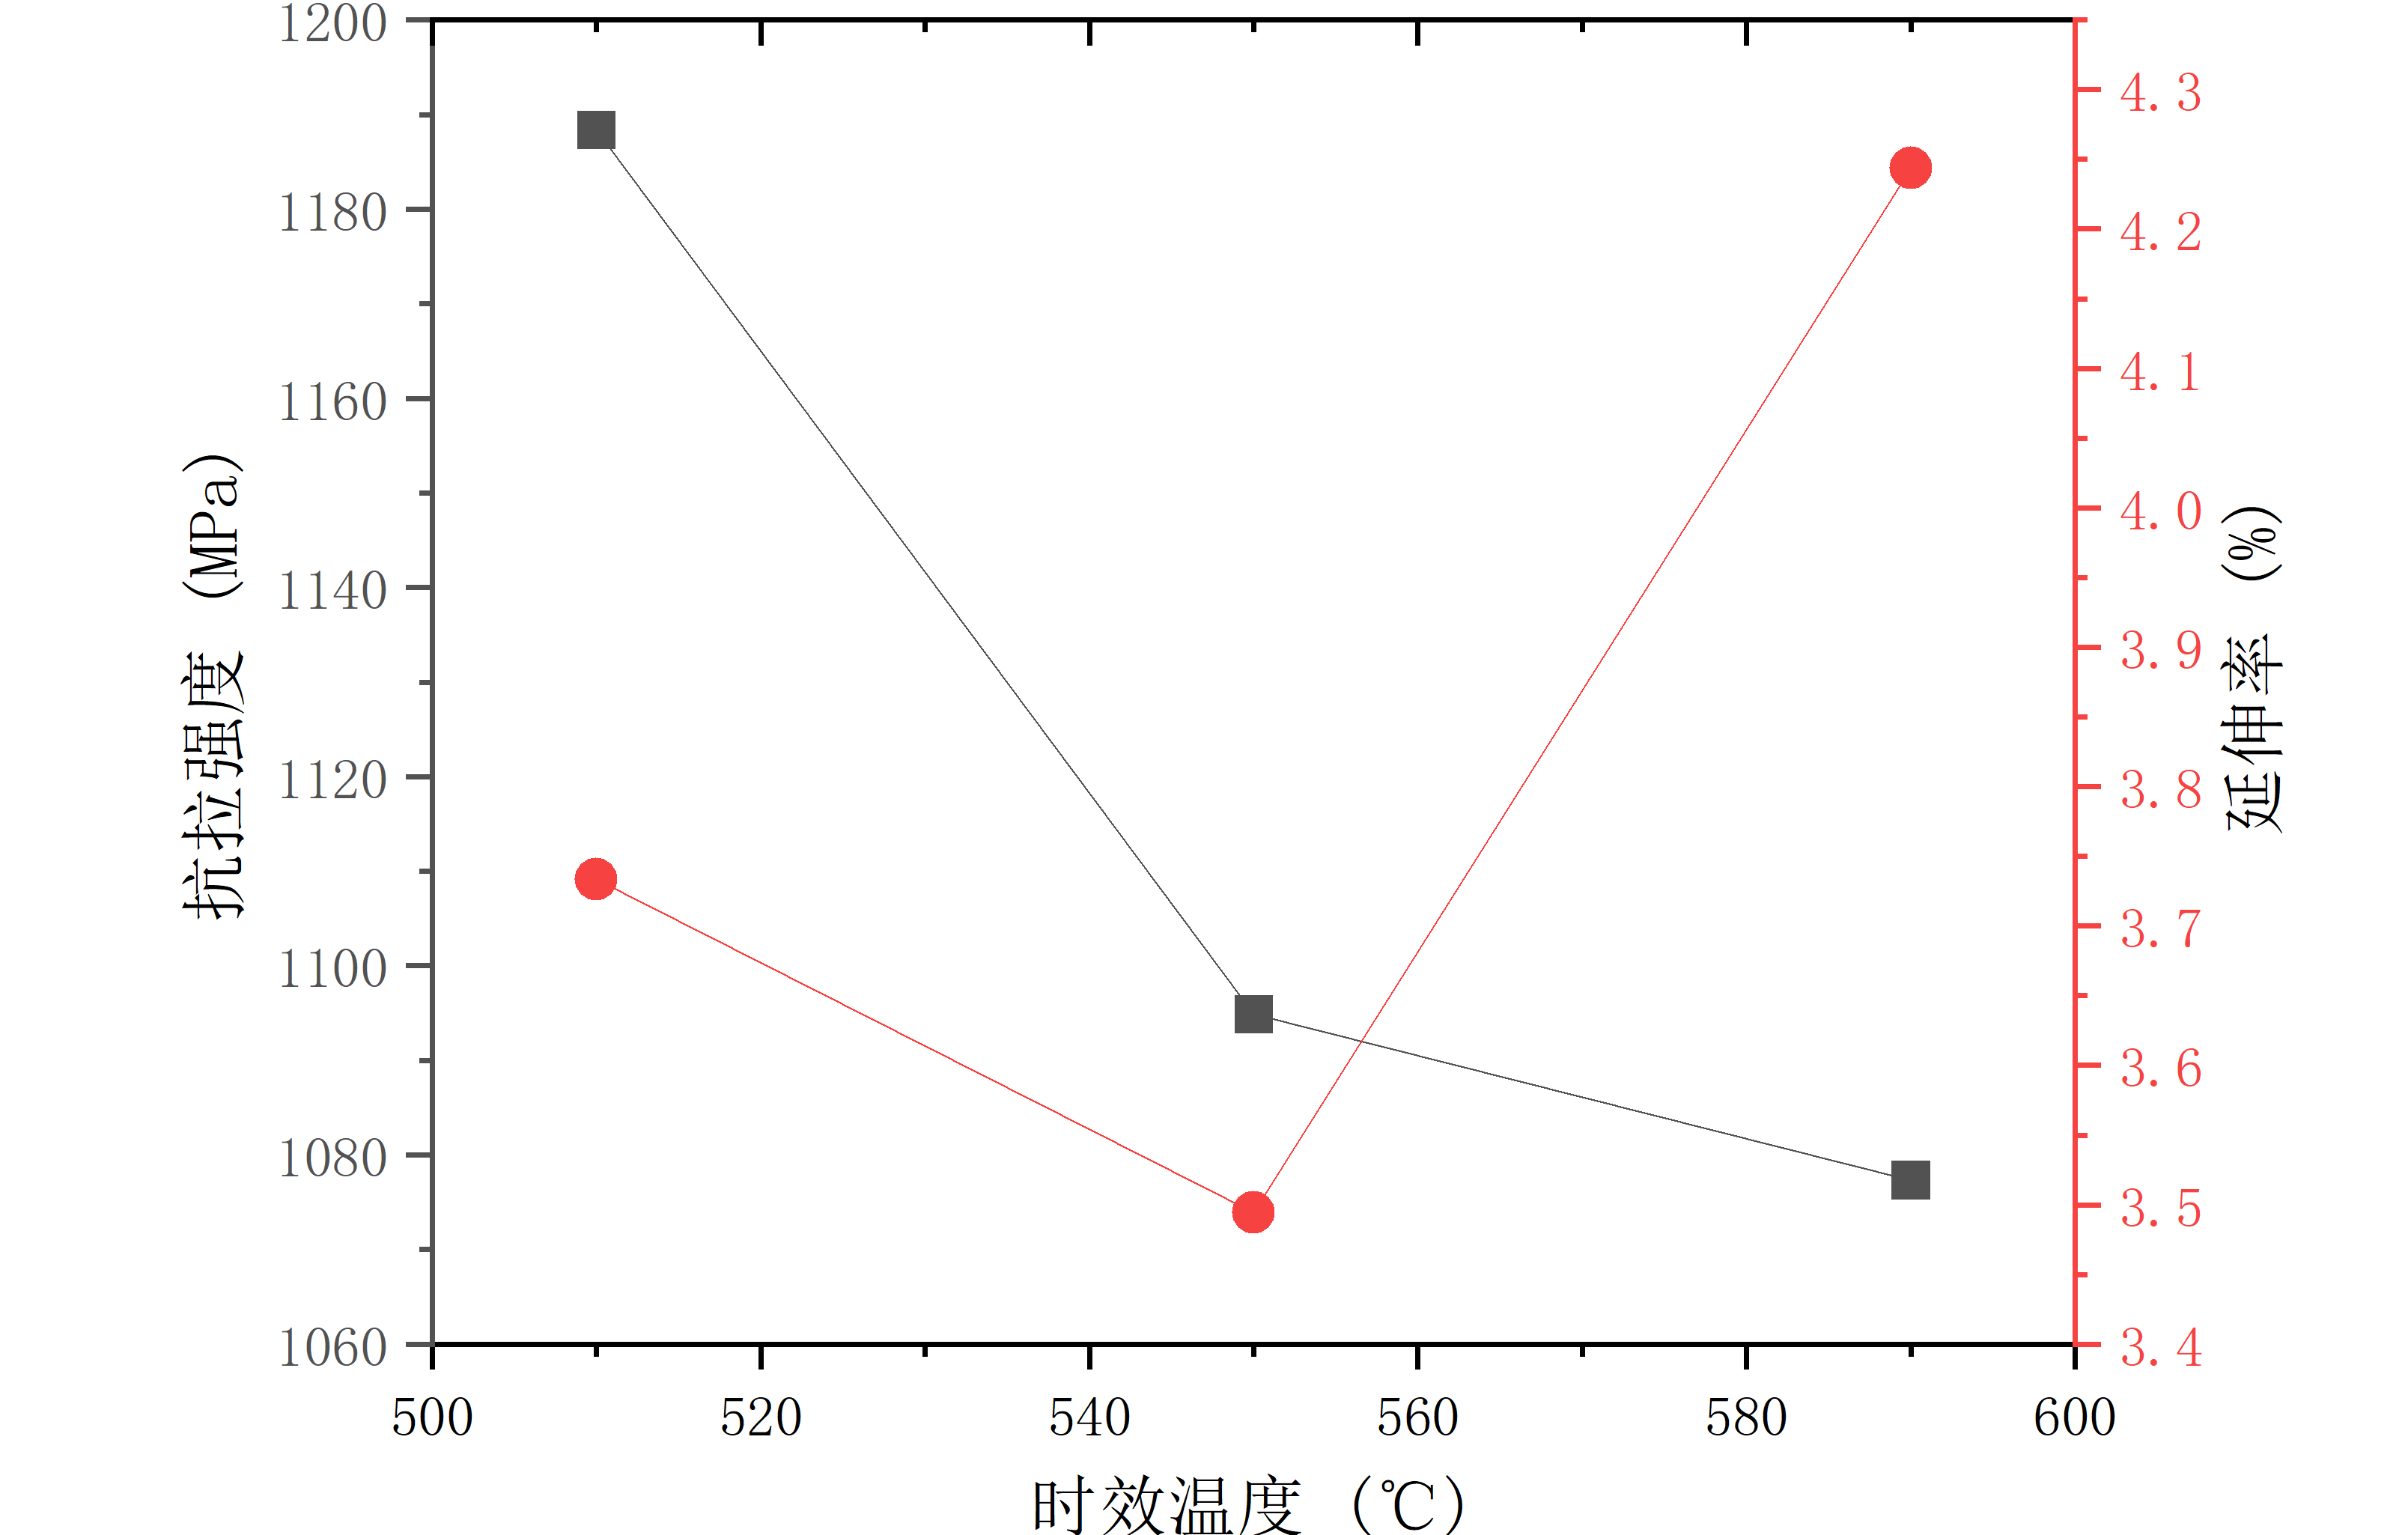
\includegraphics[width=0.7\linewidth]{pic/910分析}
			\caption{910℃固溶组的时效温度与抗拉强度、延伸率的关系}
			\label{fig:910}
		\end{figure}
			前三组试样的固溶温度为910℃,低于所用的TC4合金的相变点973℃,处于在相变点以下,时效温度都在$ 500\sim 600$℃之间。组织形貌如\ref{910}所示。

			\textbf{\faSchlix 组织分析:}在处理过程中,随着温度的升高,$ \alpha $相逐渐向$ \beta $相转变,在达到设定的温度时,组织由初生等轴$ \alpha $相和$ \beta $相组成。经过水或淬火油的快速冷却后,组织发生马氏体转变,由图\ref{fig:910510}可见,冷却后的组织有等轴初生$ \alpha $相和针状马氏体组成。

			\textbf{\faTools 性能分析:}该组试样的一个典型特点是固溶后的初生等轴$\alpha $相含量较多,而钛合金经过固溶时效后的塑性性能指标主要取决于初生等轴$\alpha $相的含量及分布\cite{zouhaibeiTC4taihejinrechuliqianghuagongyijixiangbianhangweiyanjiu2019},当初生等轴$\alpha $相的含量为$ 15\%\~20\% $之间时,随着等轴$\alpha $相的增加,材料的塑性逐渐增加,从图可以看出,该组材料的延伸率基本上达到了$ 3\% $以上,塑性较好。

			\textbf{\faThinkPeaks 固溶冷速:}由于油冷情况下的冷却速度比水冷的小,组织中的初生$\alpha $相的生长时间更久,形成的等轴$\alpha $相尺寸较大,$\beta $相中合金元素可以发生扩散,发生扩散型相变,最终形成与珠光体类似的$\alpha $片层与$\beta $片层相间分布的$\beta $转变组织,亦即双态组织;而水冷的速度比较快,本设计所用小试样的比表面积相对较大,导致冷却极快,导致$\beta \to\alpha $的扩散型相变来不及发生,$\beta $相只能通过类似马氏体相变的非扩散型晶格切变来进行相变,生成了$\alpha^{\prime}$马氏体,水冷后最终组织中含有$\alpha $相与$\alpha^{\prime} $相。

			\textbf{\faThermometerQuarter 时效温度:}由\ref{fig:910}可得,经过910℃固溶10min后水冷的合金在500℃到600℃内时效60min后,强度得到了明显提升,但塑性有所下降。而且时效温度越高,抗拉强度越低,延伸率则先减小后增大,其中抗拉强度在510℃固溶时达到最大,为1138Mpa,延伸最大600℃时的$ 3.73\% $,与对照组相比,强度上升了17.81$ \% $,延伸率下降了$ 45.33\% $。
			\newpage
\section{两相区固溶处理对组织性能的影响}

\begin{figure}[htbp]
	\centering
	\subfigure[950℃固溶(油冷)+550℃固溶]{
		\begin{minipage}[t]{0.33\linewidth}
			\centering
			
\includegraphics[width=0.9\linewidth]{pic/组织分析/950+550}
			\label{fig:950550}
		\end{minipage}%
	}%
	\subfigure[950℃固溶(水冷)+590℃固溶]{
		\begin{minipage}[t]{0.33\linewidth}
			\centering
			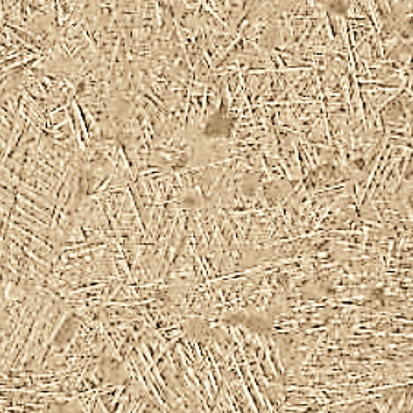
\includegraphics[width=0.9\linewidth]{pic/组织分析/950+590}
			\label{fig:950590}
			%\caption{fig2}
		\end{minipage}%
	}%
	\subfigure[950℃固溶(水冷)+510℃固溶]{
		\begin{minipage}[t]{0.33\linewidth}
			\centering
			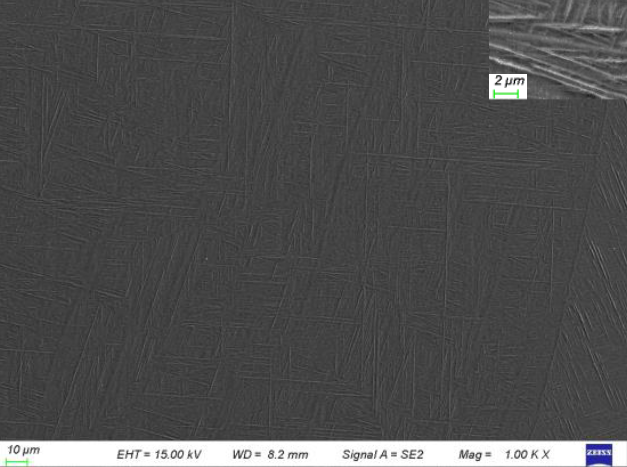
\includegraphics[width=0.9\linewidth]{pic/组织分析/950+510}
			\label{fig:950510}
			%\caption{fig2}
		\end{minipage}%
	}%
	\centering
	\label{950}
	\caption{双相区固溶的 TC4 钛合金显微组织}
\end{figure}

		\begin{figure}[h!]
			\centering
			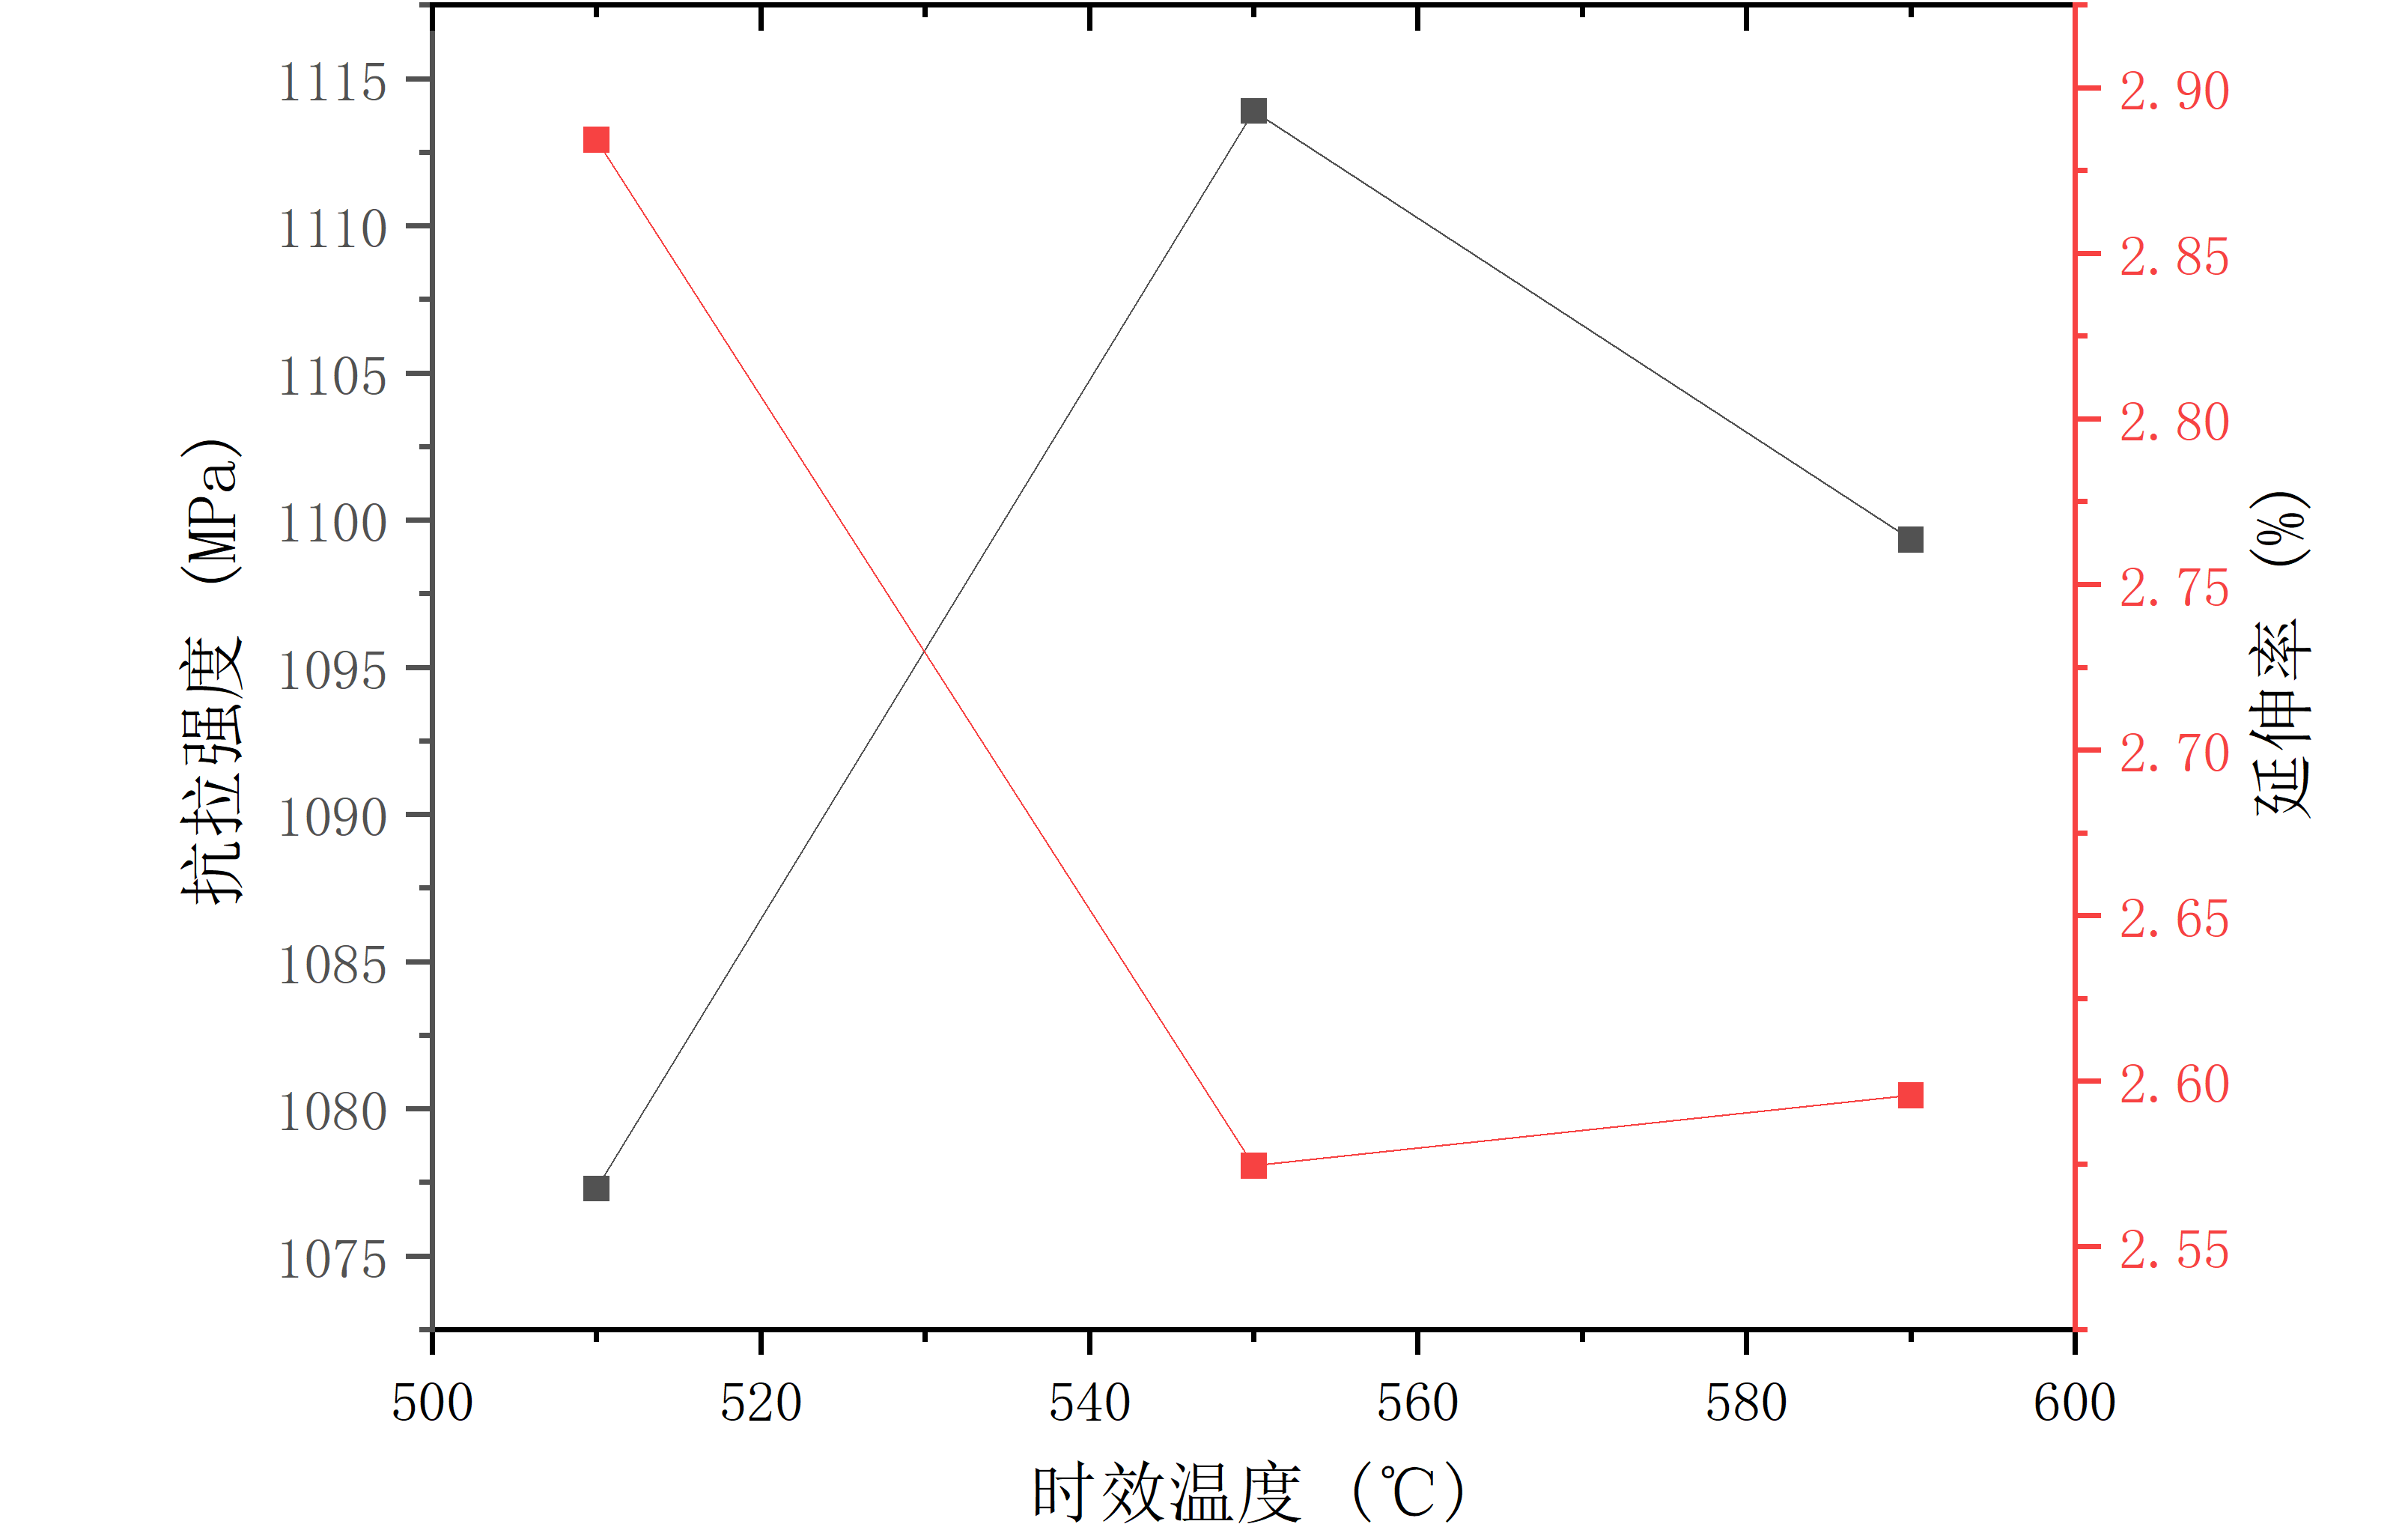
\includegraphics[width=0.7\linewidth]{pic/950分析}
			\caption{950分析}
			\label{fig:950}
		\end{figure}

\textbf{\faSchlix 组织分析:}如\ref{fig:950590}所示:在$ \alpha+\beta $两相区进行固溶后水冷,得到初生等轴$ \alpha $相与细针状$ \alpha^{\prime}$马氏体交错组成的双态组织,与第一大组相比,由于加热温度偏高,$ \beta $相长大,形成的$ \beta $相比较粗大。

\textbf{\faTools 性能分析:}从\ref{950}可以看出,这三组的抗拉均强度明显高于对照组,说明经过固溶和时效处理后,钛合金的综合力学性能得到了提升。然而延伸率却明显降低,说明处理后材料的塑性变差。

\textbf{\faThinkPeaks 固溶冷速:}水冷的冷却速度比油冷快,导致材料的强化相数量增多,也会导致较大的晶粒尺寸。而油冷则相反,会产生更细小的强化相和晶粒。

\textbf{\faThermometerQuarter 时效温度:}由\ref{fig:950}可得,时效温度越高,亚稳定$ \beta $相的分解越充分,可以得到较好的强度与塑韧性,但当时效温度过高时,组织变粗大,性能较差。

\section{相变点以上固溶处理对组织性能的影响}
如\ref{fig:990590}所示:在$ \alpha+\beta $两相区进行固溶后冷却,得到粗大的原始$ \beta $相晶粒内部分布着单一的细针状马氏体,
\begin{figure}[htbp]
	\centering
	\subfigure[990℃固溶(水冷)+550℃固溶]{
		\begin{minipage}[t]{0.33\linewidth}
			\centering
			
\includegraphics[width=0.9\linewidth]{pic/组织分析/990+550}
			\label{fig:990550}
		\end{minipage}%
	}%
	\subfigure[990℃固溶(水冷)+590℃固溶]{
		\begin{minipage}[t]{0.33\linewidth}
			\centering
			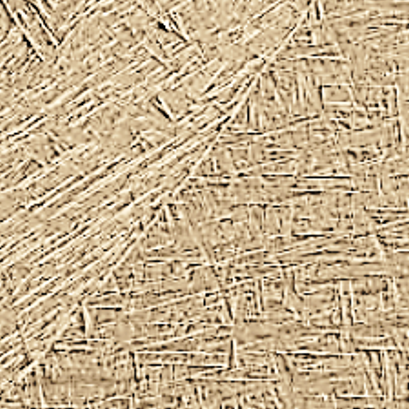
\includegraphics[width=0.9\linewidth]{pic/组织分析/990+590}
			\label{fig:990590}
			%\caption{fig2}
		\end{minipage}%
	}%
	\subfigure[990℃固溶(油冷)+510℃固溶]{
		\begin{minipage}[t]{0.33\linewidth}
			\centering
			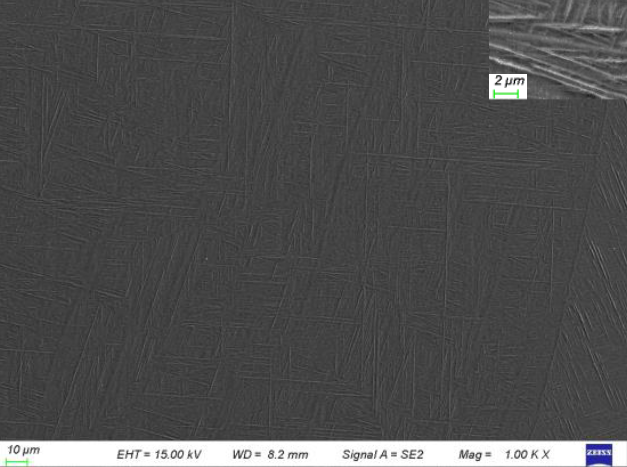
\includegraphics[width=0.9\linewidth]{pic/组织分析/990+510}
			\label{fig:990510}
			%\caption{fig2}
		\end{minipage}%
	}%
	\centering
	\caption{双相区固溶的 TC4 钛合金显微组织}
\end{figure}

\begin{figure}[h!]
	\centering
	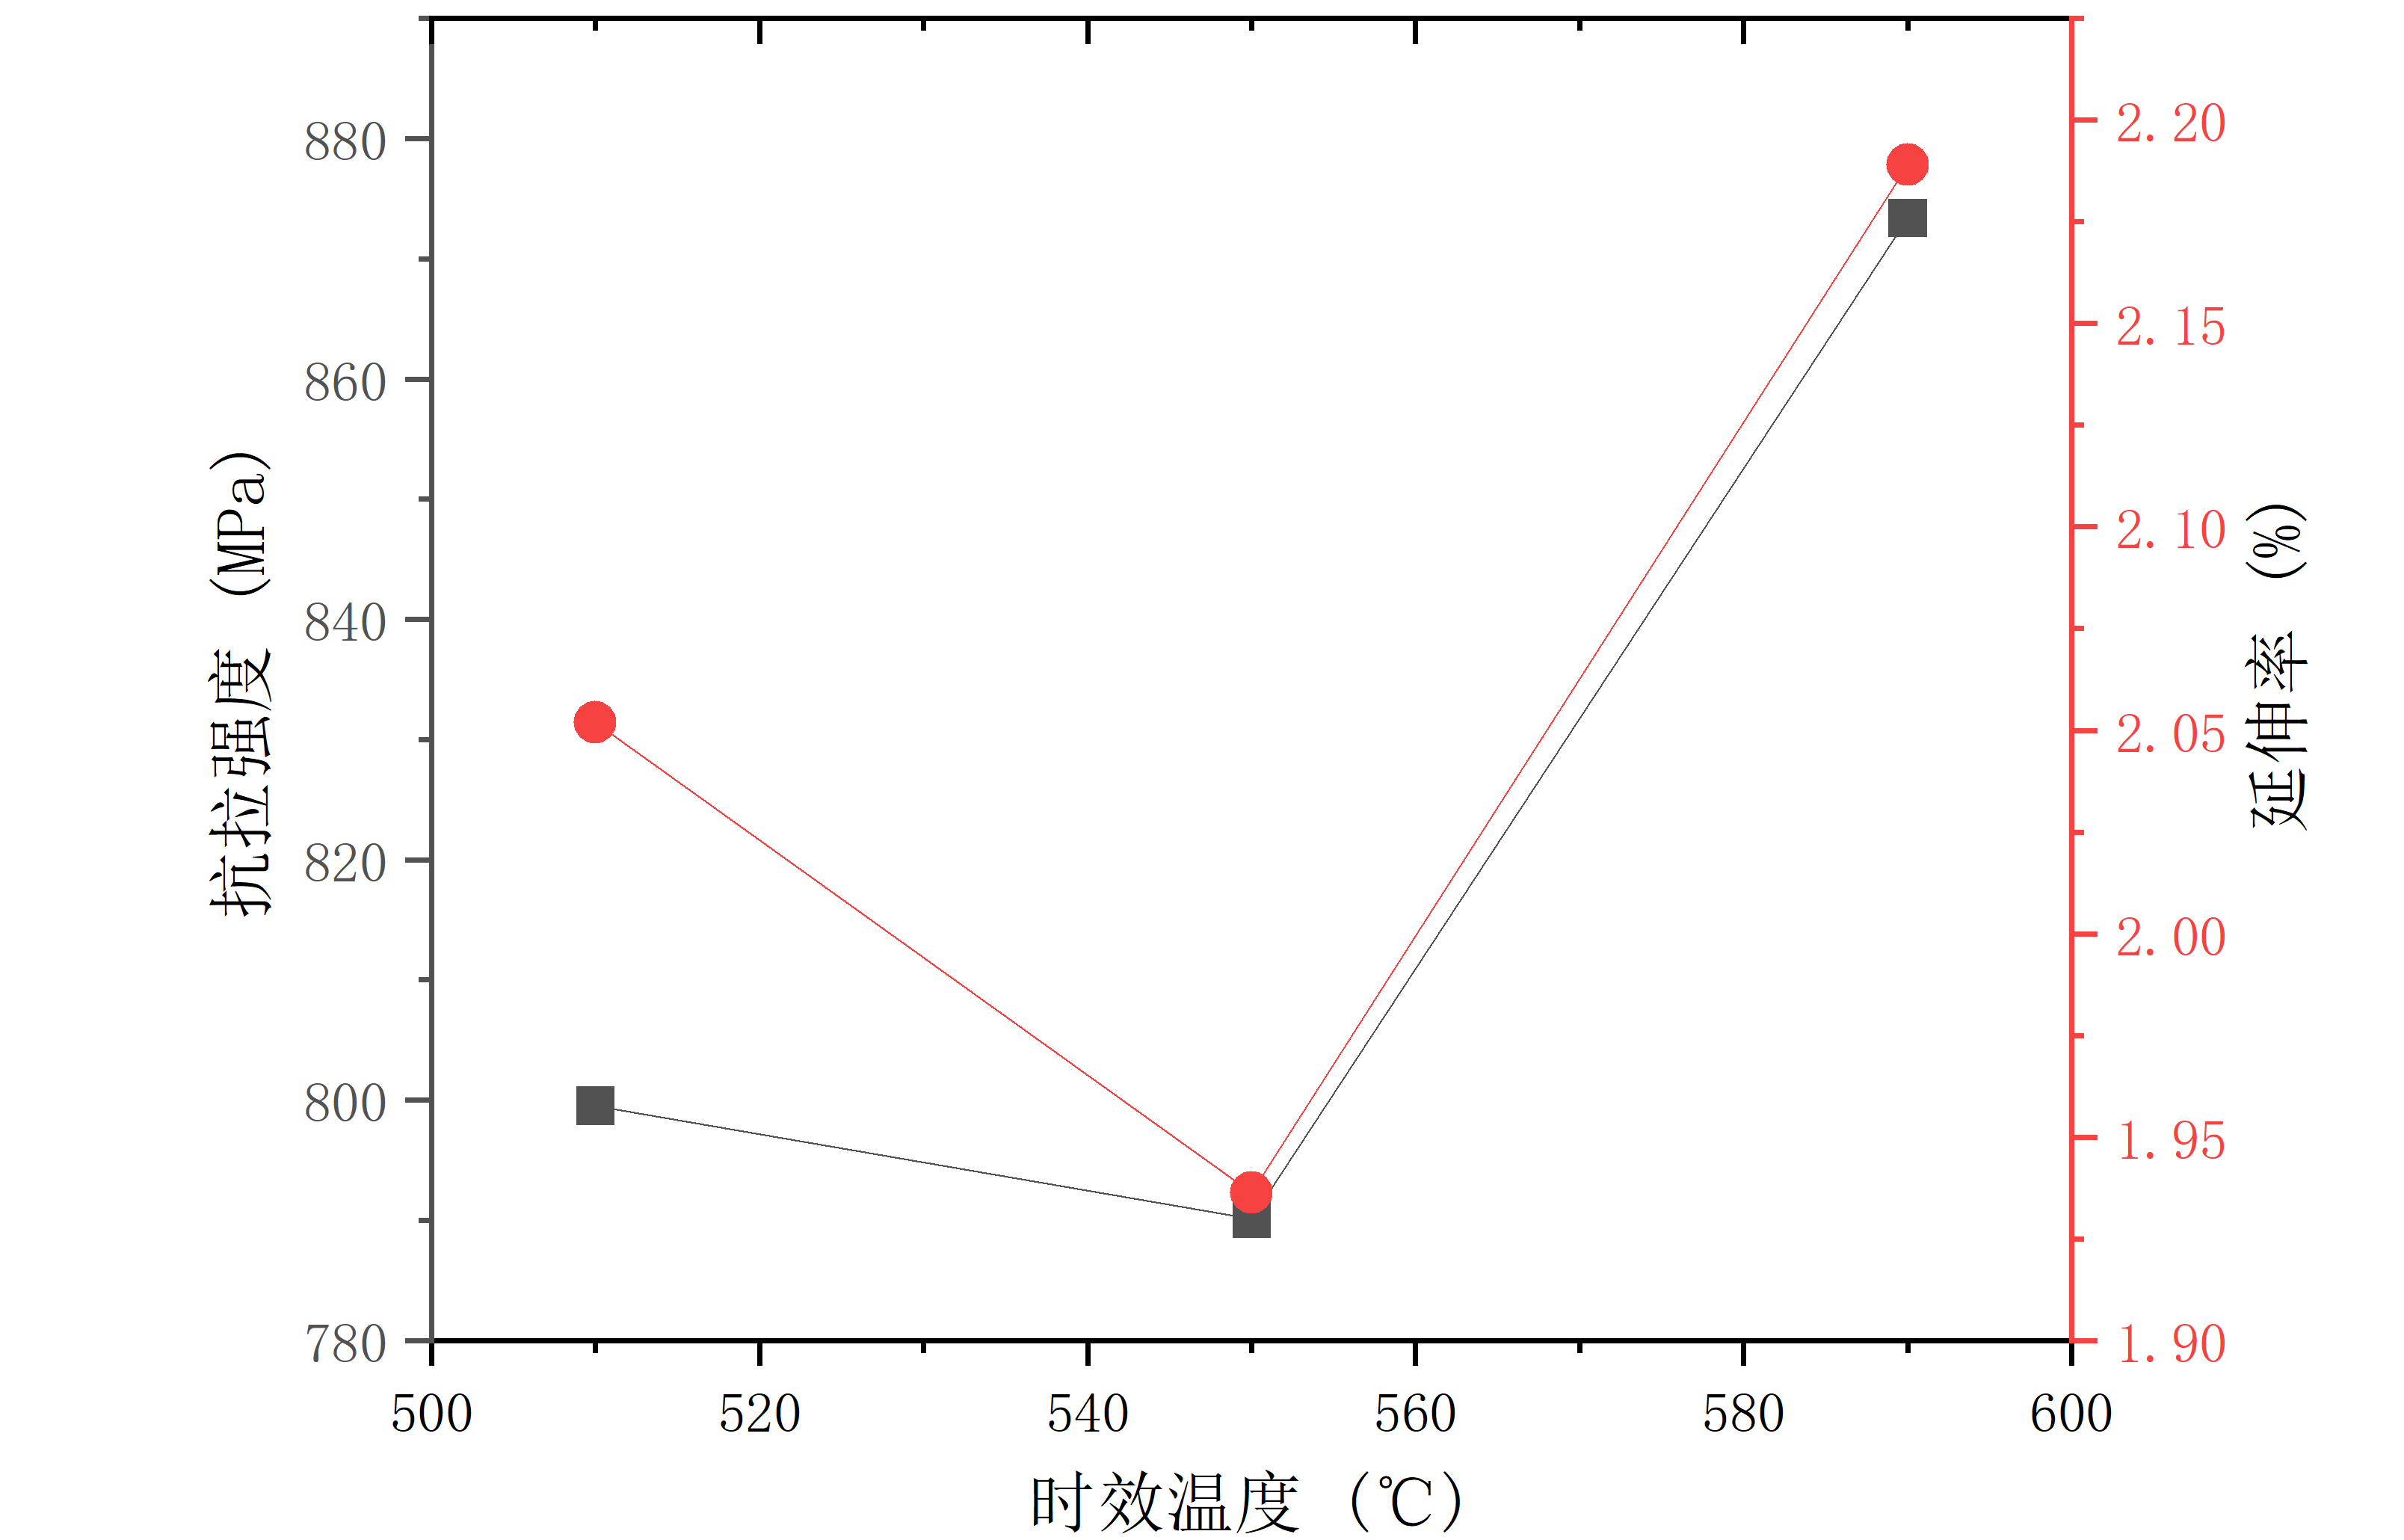
\includegraphics[width=0.7\linewidth]{pic/970分析}
	\caption{970分析}
	\label{fig:970}
\end{figure}




\section{正交实验分析}
本设计通过正交实验饭进行实验的设计,通过正交实验法得到的固溶温度、冷却方式、时效温度与抗拉强度的关系如下:
\begin{table}[htbp]
	\centering
	\caption{固溶温度、冷却方式、时效温度与抗拉强度关系表}
	\label{sec:zjq}
	\begin{tabular}{cccccc}
		\toprule
		 差异源 & 平方和 & df & 均方 & F & p \\
		 	\midrule
Intercept & 8078602.799 & 1 & 8078602.799 & 3561.305 & 0.000** \\
固溶温度 & 166133.961 & 2 & 83066.98 & 36.619 & 0.008** \\
冷却方式 & 4354.254 & 1 & 4354.254 & 1.919 & 0.26 \\
时效温度 & 804.901 & 2 & 402.45 & 0.177 & 0.846 \\
%Residual & 6805.317 & 3 & 2268.439
		\bottomrule
	\end{tabular}
\end{table}

从上表可知,利用三因素方差分析去研究固溶温度,冷却方式和时效温度对于抗拉强度的影响关系,从上表可以看出:固溶温度呈现出显著性(F=36.619,p=0.008<0.05) ,说明主效应存在,固溶温度会对抗拉强度产生差异关系。具体差异可通过方差分析进行具体分析。冷却方式没有呈现出显著性(F=1.919,p=0.260>0.05) ,说明冷却方式并不会对抗拉强度产生差异关系。时效温度没有呈现出显著性(F=0.177,p=0.846>0.05) ,说明时效温度并不会对抗拉强度产生差异关系。

固溶温度、冷却方式、时效温度与延伸率的关系如下:
\begin{table}[htbp]
	\centering
	\caption{固溶温度、冷却方式、时效温度与延伸率关系表}
	\label{sec:zjy}
	\begin{tabular}{cccccc}
		\toprule
		差异源 & 平方和 & df & 均方 & F & p \\
		\midrule
Intercept & 0.007 & 1 & 0.007 & 2565.824 & 0.000** \\
固溶温度 & 0 & 2 & 0 & 91.373 & 0.002** \\
冷却方式 & 0 & 1 & 0 & 4.717 & 0.118 \\
时效温度 & 0 & 2 & 0 & 3.471 & 0.166 \\
Residual & 0 & 3 & 0 & ~ & ~ \\
%R 2: 0.985
		\bottomrule
	\end{tabular}
\end{table}


从上表可知,利用三因素方差分析去研究固溶温度,冷却方式和时效温度对于延伸率的影响关系,从上表可以看出:固溶温度呈现出显著性(F=91.373,p=0.002<0.05) ,说明主效应存在,固溶温度会对延伸率产生差异关系。具体差异可通过方差分析进行具体分析。冷却方式没有呈现出显著性(F=4.717,p=0.118>0.05) ,说明冷却方式并不会对延伸率产生差异关系。时效温度没有呈现出显著性(F=3.471,p=0.166>0.05) ,说明时效温度并不会对延伸率产生差异关系。
